%%%%%%%%%%%%%%%%%%%%%%%%%%%%%%%%%%%%%%%%%%%%%%%%%%%%%%%%%%%%%%%%%%%%%%%%%
% $Id$
% %%%%%%%%%%%%%%%%%%%%%%%%%%%%%%%%%%%%%%%%%%%%%%%%%%%%%%%%%%%%%%%%%%%%%%%%%
%
% Set de slides dedicadas a formulacion Ewald con 1D periodicity
%
% %%%%%%%%%%%%%%%%%%%%%%%%%%%%%%%%%%%%%%%%%%%%%%%%%%%%%%%%%%%%%%%%%%%%%%%%%

% %%%%%%%%%%%%%%%%%%%%%%%%%%%%%%%%%%%%%%%%%%%%%%%%%%%%%%%%%%%%%%%
  \subsection{Differences with Respect to 2D Periodicity}
% %%%%%%%%%%%%%%%%%%%%%%%%%%%%%%%%%%%%%%%%%%%%%%%%%%%%%%%%%%%%%%%

    \begin{frame}[fragile,allowframebreaks]{\GreenTEw}

    
    \begin{block}{Ewald Method in HOFEM}
    \begin{columns}[T]
      \column{0.50\textwidth}
      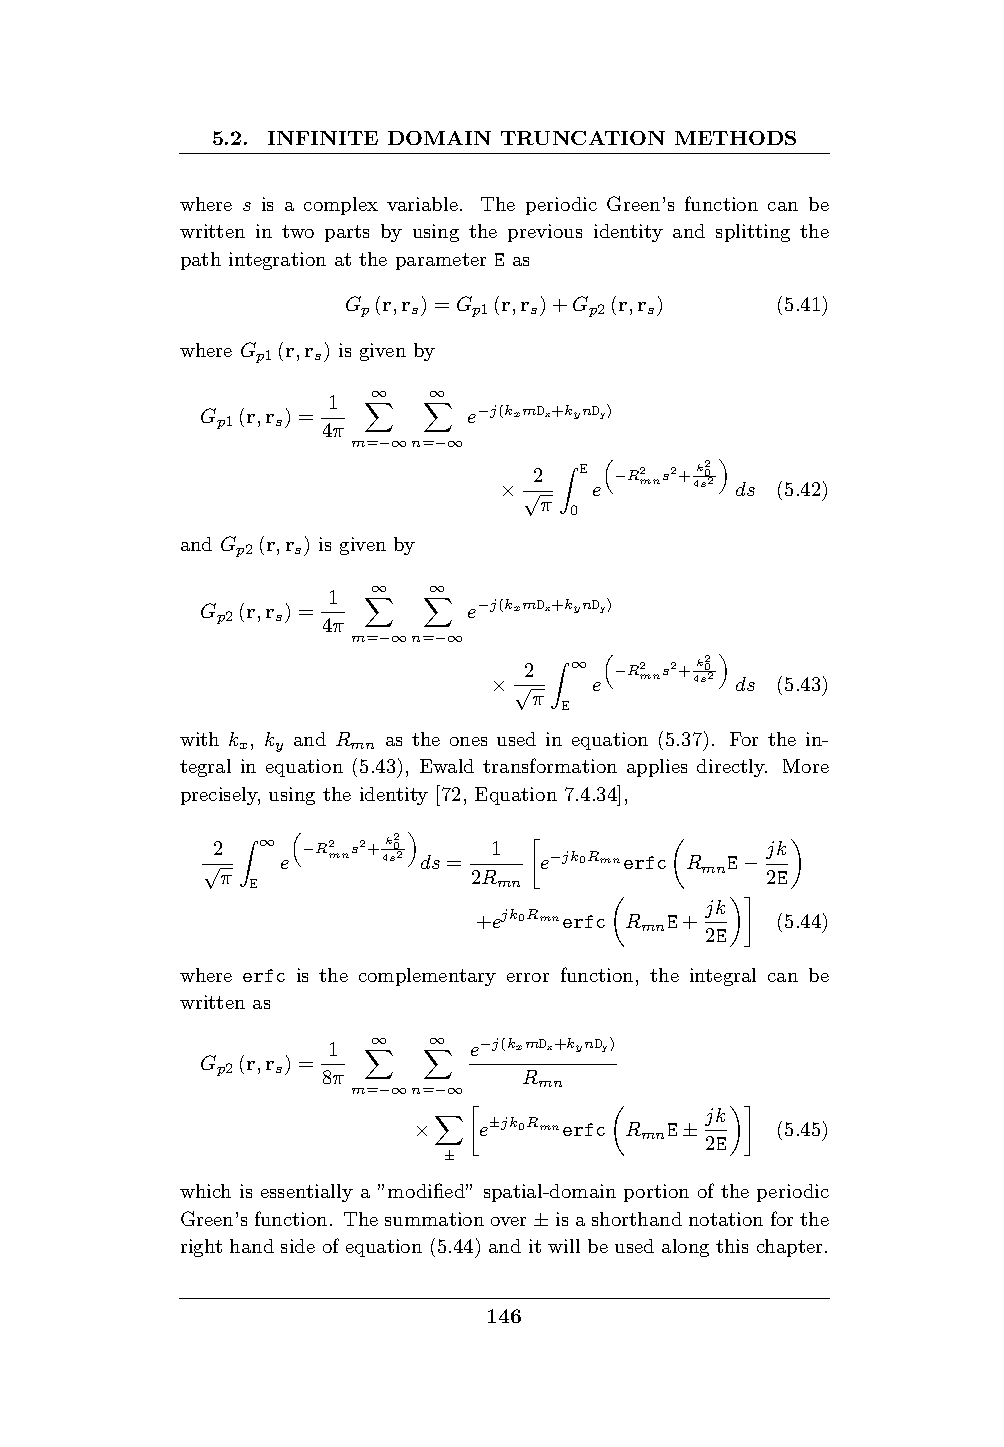
\includegraphics[width=\textwidth,clip=true,trim=70 350 70 80]{Tesis_Daniel_Ewald_1} 
      \column{0.45\textwidth}
      \begin{lstlisting}[style=myFORTRANcodeS,basicstyle=\ttfamily\tiny]
!Distancia de la celda unidad en X
 Dx = SQRT(DOT_PRODUCT(PBC_structure%offset_vector(1,:),PBC_structure%offset_vector(1,:)))
 !Distancia de la celda unidad en Y
 Dy = SQRT(DOT_PRODUCT(PBC_structure%offset_vector(2,:),PBC_structure%offset_vector(2,:)))
    
 E = SQRT(PI/Dx/Dy)

 !Sum using Ewald transformation
 DO m=-2,2
    DO n=-2,2

    !Calcular alpha_mn
    alpha_mn = SQRT(CMPLX((PI*m/Dx)**2 + (PI*n/Dy)**2 + (PI*m/Dx)*Kx + &
    (PI*n/Dy)*Ky + (1.0_DBL/4.0_DBL)*(Kx**2+Ky**2-K**2),0.0_DBL,KIND=DBL));
      \end{lstlisting}
    \end{columns}
  \end{block}


  \begin{block}{Ewald 1D periodicity}
    \begin{itemize}
    \item Naively we thought if was simply setting
      either $m=0$ or $n=0$
    \item \alert{But it is NOT} \ldots
%      \hyperlink{Ewald1D}{click here to go to section on Ewald 1D}
      \hyperlink{Ewald1D}{see next slided on Ewald 1D}
    \end{itemize}
  \end{block}

  \end{frame}

  % %%%%%%%%%%%%%%%%%%%%%%%%%%%%%%%%%%%%%%%%%%%%%%%%%%%%%%%%%%%%%%%
      \usetikzlibrary {arrows.meta}
  
\begin{frame}[allowframebreaks]{Ewald sum}

  \begin{itemize}
    \item Technique for summing contribution from an infinite set of sources (in 
      this case along $z$ axis):
      \[
        \sum_n G(R_n) = 
        \frac{1}{4\pi}\sum_n
        e^{-j(k\cos\theta)nd}
        \frac{e^{-jkR_n}}{R_n}
      \]
      \small
      where 
      $R_n=\sqrt{(x-x')^2 + (y-y')^2 + (z-z'+nd)^2}$, $\theta$ is elevation 
      angle.
    \item The Green function is decomposed in two terms:
      \[
        \sum_n G(R_n) = \sum_n G_1(R_n) + \sum_n G_2(R_n)
      \]
      \begin{itemize}
        \item One of them decays quickly with $R_n$: $|G_2(R_{n+1})| \ll |G_2(R_{n})|$
        \item For the other one the 
          \href{https://en.wikipedia.org/wiki/Poisson_summation_formula}
          {Poisson summation formula}
          is applied:
          \[
            \sum_n G_1(R_n) = \sum_n \hat{G}_1(k_n)
          \]

          \vspace{-2ex}
          where $\hat{G}_1(k)$ is the Fourier transform of $G_1(R)$%
          \footnote{$\hat{G}_1(k)$ is narrow in $k$ because $G_1(R)$ is wide in $R$}.

      \end{itemize}

  \end{itemize}

  
\end{frame}
  
% %%%%%%%%%%%%%%%%%%%%%%%%%%%%%%%%%%%%%%%%%%%%%%%%%%%%%%%%%%%%%%%

\begin{frame}[allowframebreaks]{1D from 2D periodicity Ewald sum}

  \begin{itemize}
    \item No problem with \emph{spatial} term:
      \[
        \sum_m\sum_n G_2(R_{n,m}) \rightarrow \sum_{n} G_2(R_{n,0})
      \]
    \item But the \emph{spectral} term...
      \[
        \sum_m\sum_n \hat{G}_1(k_{n,m}) \rightarrow ??
      \]

      The Fourier Transform of $G_1(n,0)$ must be computed from scratch:

      \begin{gather*}
        \hat{G}_{1,n} =
        \frac{e^{j(z-z')(k_z - 2\pi \frac{n}{d})}}{2 \pi d} 
        g\left(\frac{\alpha_n^2}{4 E^2}, \rho^2 E^2\right)
        \\
         \rho^2 = (x-x')^2 + (y-y')^2
         \qquad
         \alpha_n^2 = \left(k\cos\theta + \frac{2 \pi n}{d}\right)^2 - k^2
      \end{gather*}
      where we need the following numerical integration
      \[
        g(a,b) = \int_0^1 \frac{
          e^{-\frac{a}{z^2}-b z^2}
        }{z}
        \, dz
      \]
  \end{itemize}

\end{frame}

% %%%%%%%%%%%%%%%%%%%%%%%%%%%%%%%%%%%%%%%%%%%%%%%%%%%%%%%%%%%%%%%

\begin{frame}[allowframebreaks]{Notes about g(a,b)}
  \begin{itemize}
    \item It is a complex integral whose value (and convergence) depends on the chosen path.
    \item For calculating $\hat{G}_{1,n}$:
      \begin{itemize}
        \item $a,b \in \mathbb{R}$
        \item $b>0$, 
        \item but $a$ is negative for the first $n$ values (At each $n$ term in 
          the sum $a=\alpha_n^2/4E^2$).
      \end{itemize}
    \item If $a>0$, the integral can be done through real axis.
    \item If $a<0$, the integral must be done through the following path:

      \vbs

      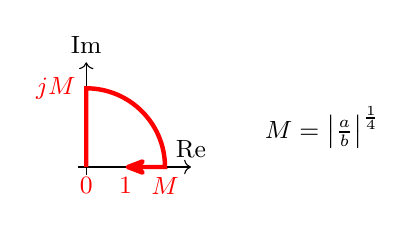
\begin{tikzpicture}[node font=\small]
        \draw[->] (-0.1,0) -- (1.33,0) node[above] {Re};
        \draw[->] (0,-0.1) -- (0,1.33) node[above] {Im};
        \draw[red, ultra thick, arrows={-Stealth[round]}] 
          (0,0) node [below] {$0$} -- (0,1) node[left] {$jM$} 
        arc[start angle=90, end angle=0, radius=1] node[below] {$M$}
        -- (0.5,0) node[below] {$1$}
        ;
        \node at (3,0.5) {$M=\left|\frac{a}{b}\right|^{\frac{1}{4}}$};
      \end{tikzpicture}

    \item If $a=0$, integral does not converge. It happens for specific values 
      of $k$ and $d$ (not a problem: Greens function is singular there).
  \end{itemize}
\end{frame}

% %%%%%%%%%%%%%%%%%%%%%%%%%%%%%%%%%%%%%%%%%%%%%%%%%%%%%%%%%%%%%%%

\begin{frame}{Checking results (thin slice)}
  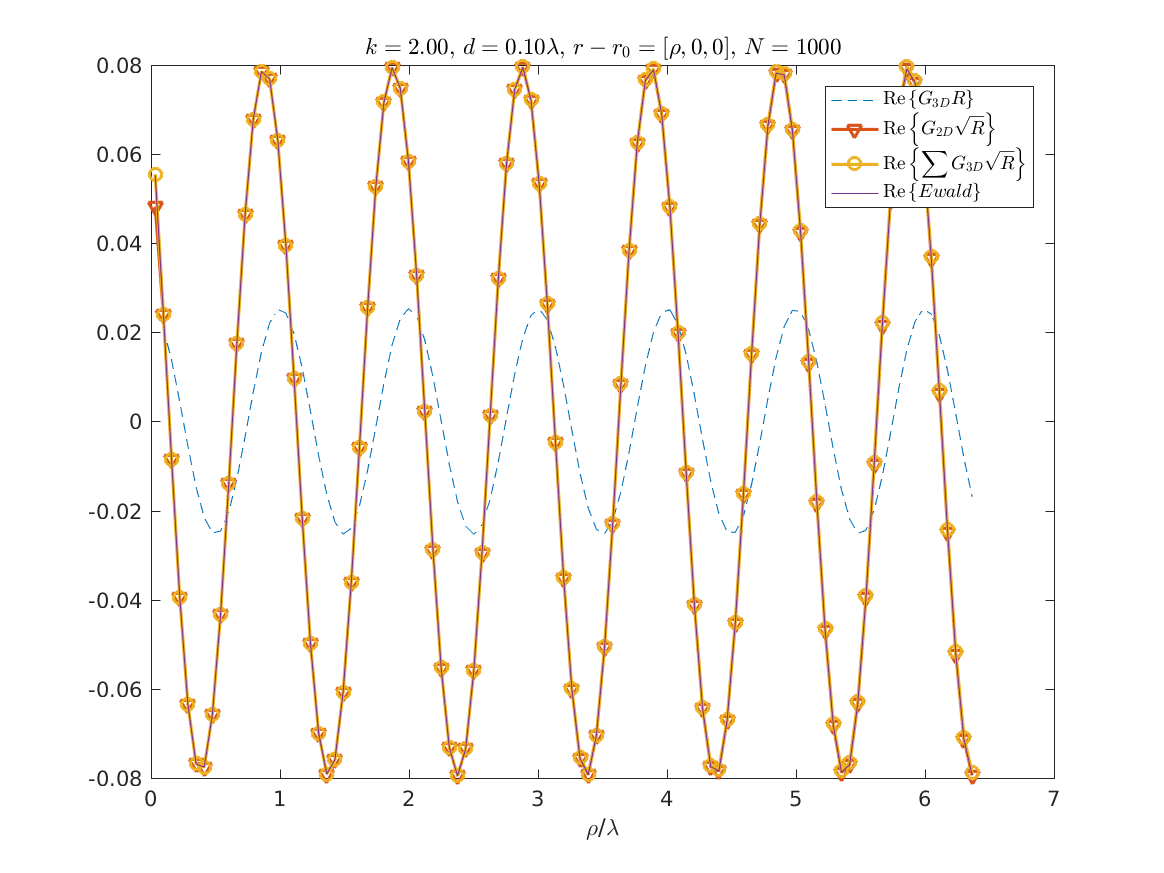
\includegraphics[width=0.9\textwidth]{GreenFunctions_R_ew1.png}
\end{frame}
\begin{frame}{Checking results (medium slice)}
  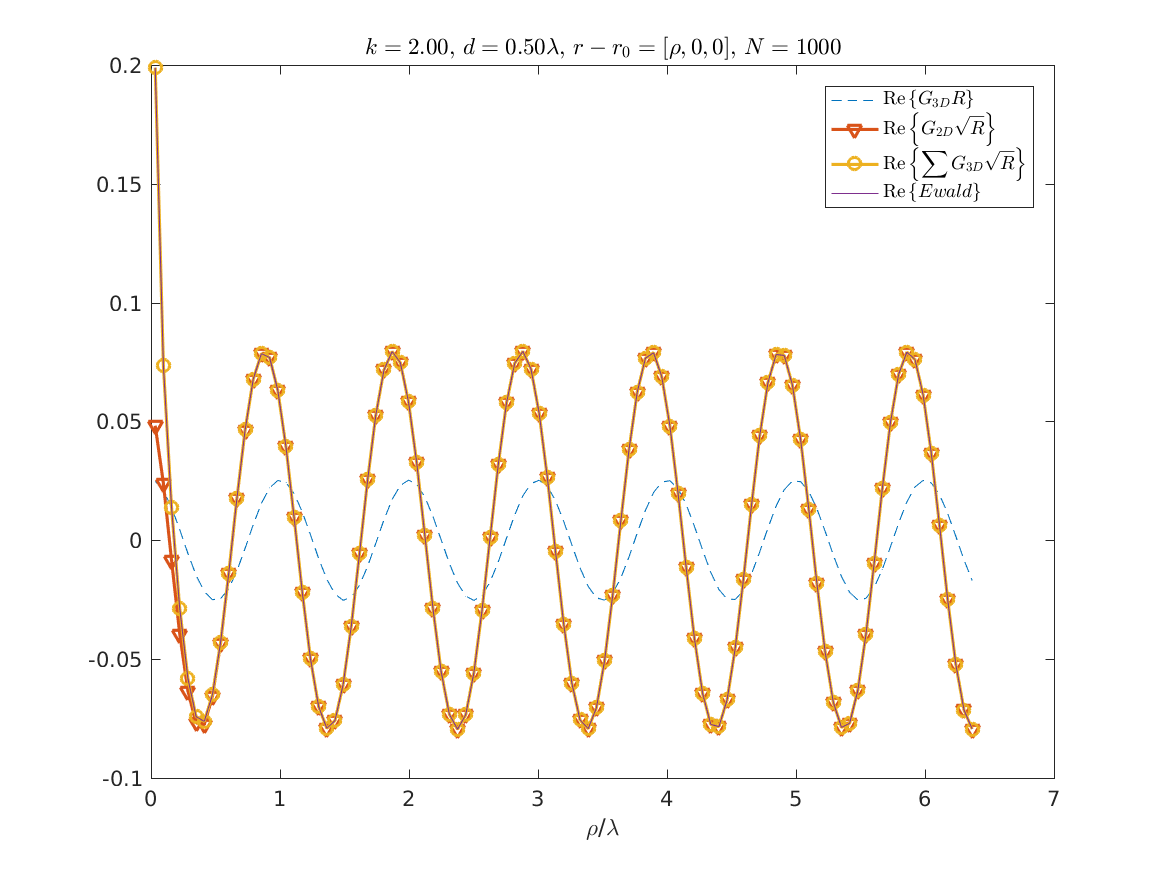
\includegraphics[width=0.9\textwidth]{GreenFunctions_R_ew2.png}
\end{frame}
\begin{frame}{Checking results (thick slice)}
  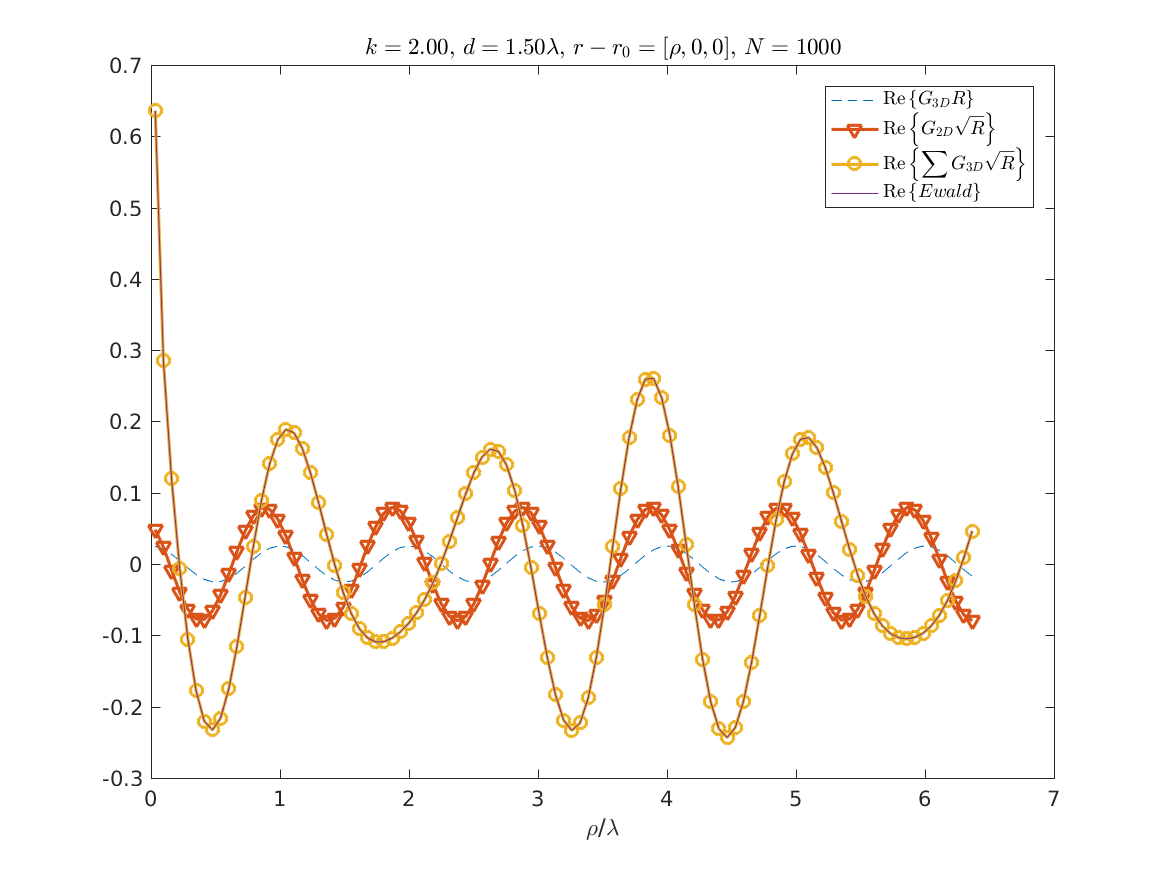
\includegraphics[width=0.9\textwidth]{GreenFunctions_R_ew3.png}
\end{frame}
\begin{frame}{Checking results (close to transverse Floquet resonance)}{$\alpha^2_0 \simeq 0$}
  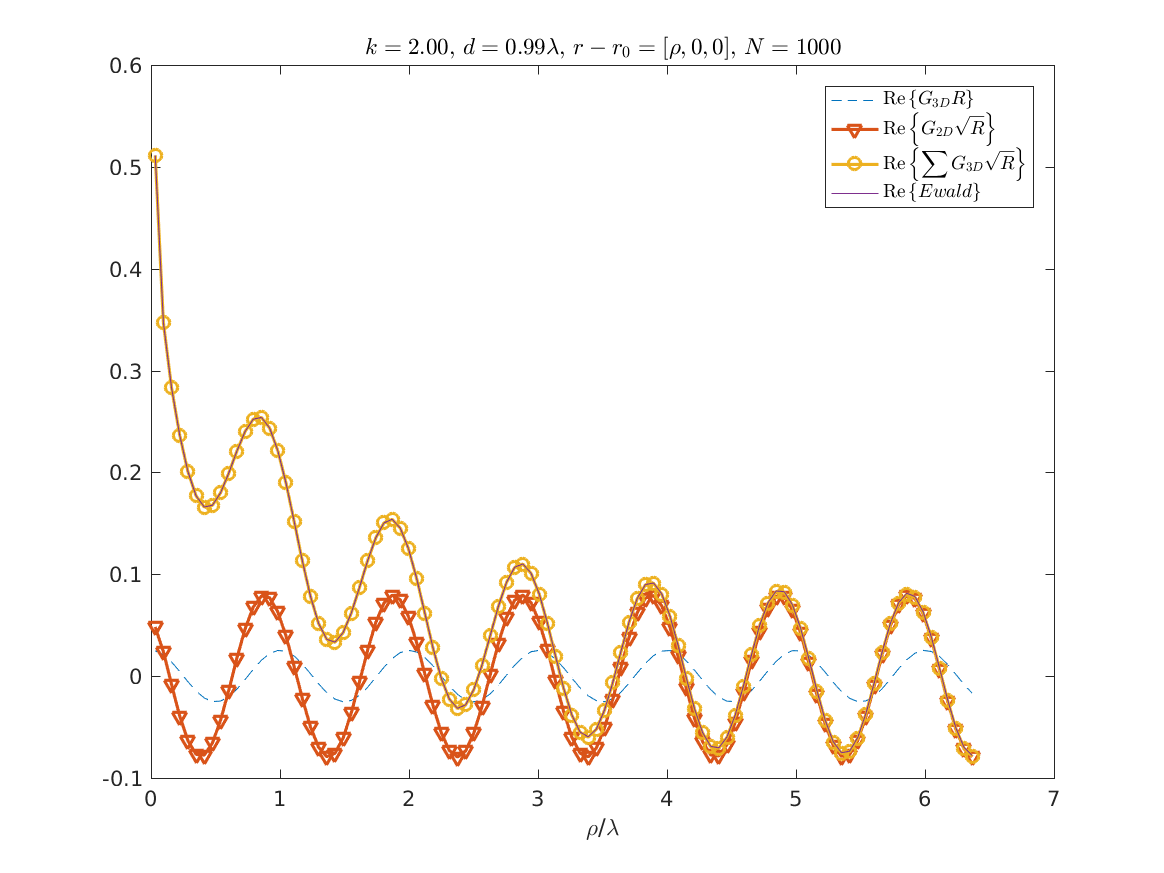
\includegraphics[width=0.9\textwidth]{GreenFunctions_R_ew_P0.png}
\end{frame}
\begin{frame}{Checking results (close to transverse Floquet 
  resonance)}{$\alpha^2_0 \simeq 0$}
  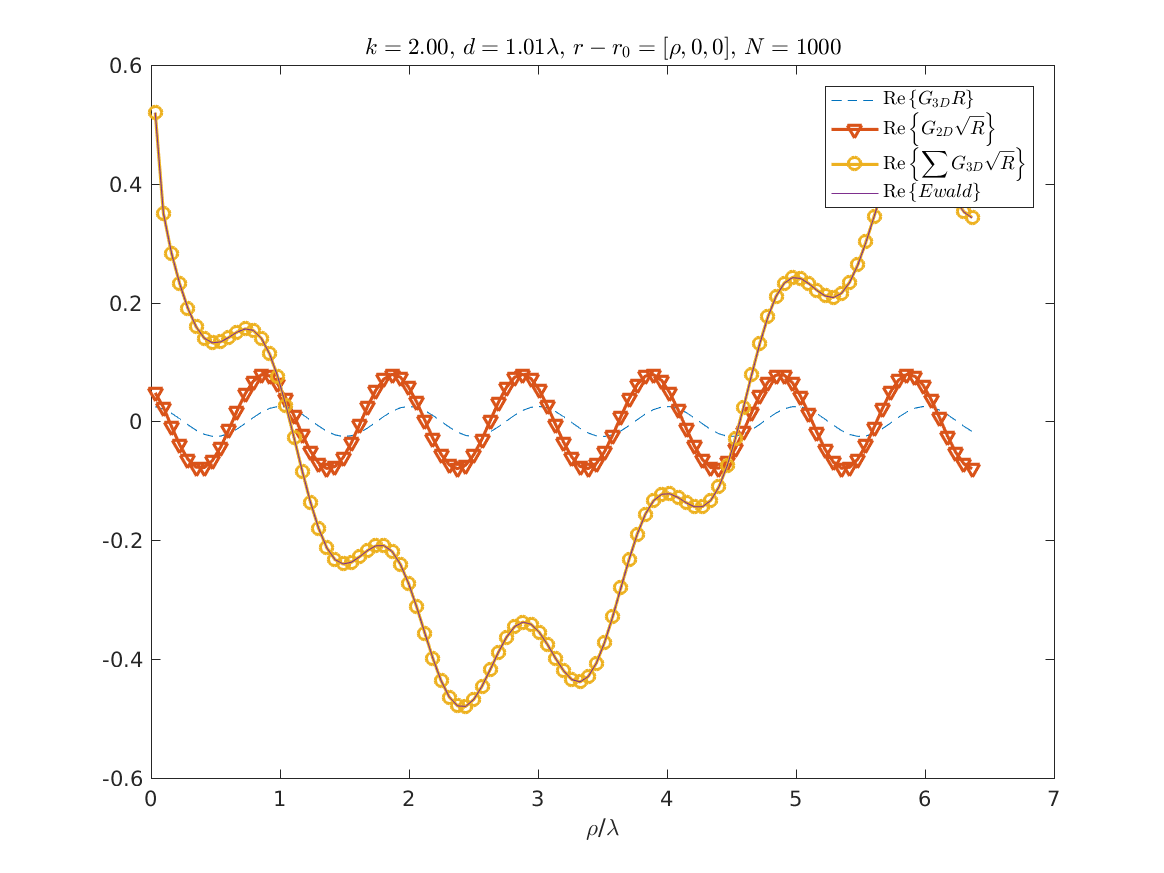
\includegraphics[width=0.9\textwidth]{GreenFunctions_R_ew_P1.png}
\end{frame}
\begin{frame}[allowframebreaks]{Convergence of the direct sum}

  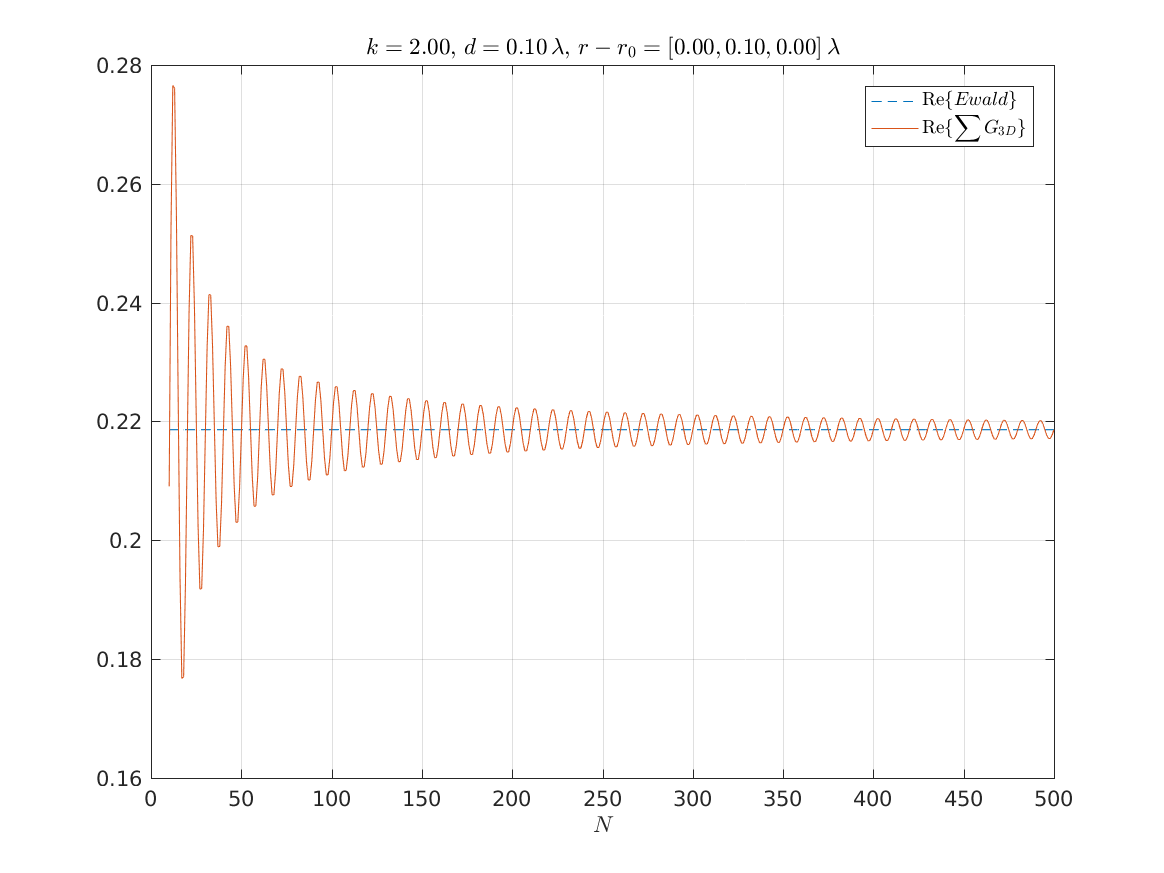
\includegraphics[width=0.8\textwidth]{GreenFunctions_convN_re_ew01.png}
 
  \framebreak

  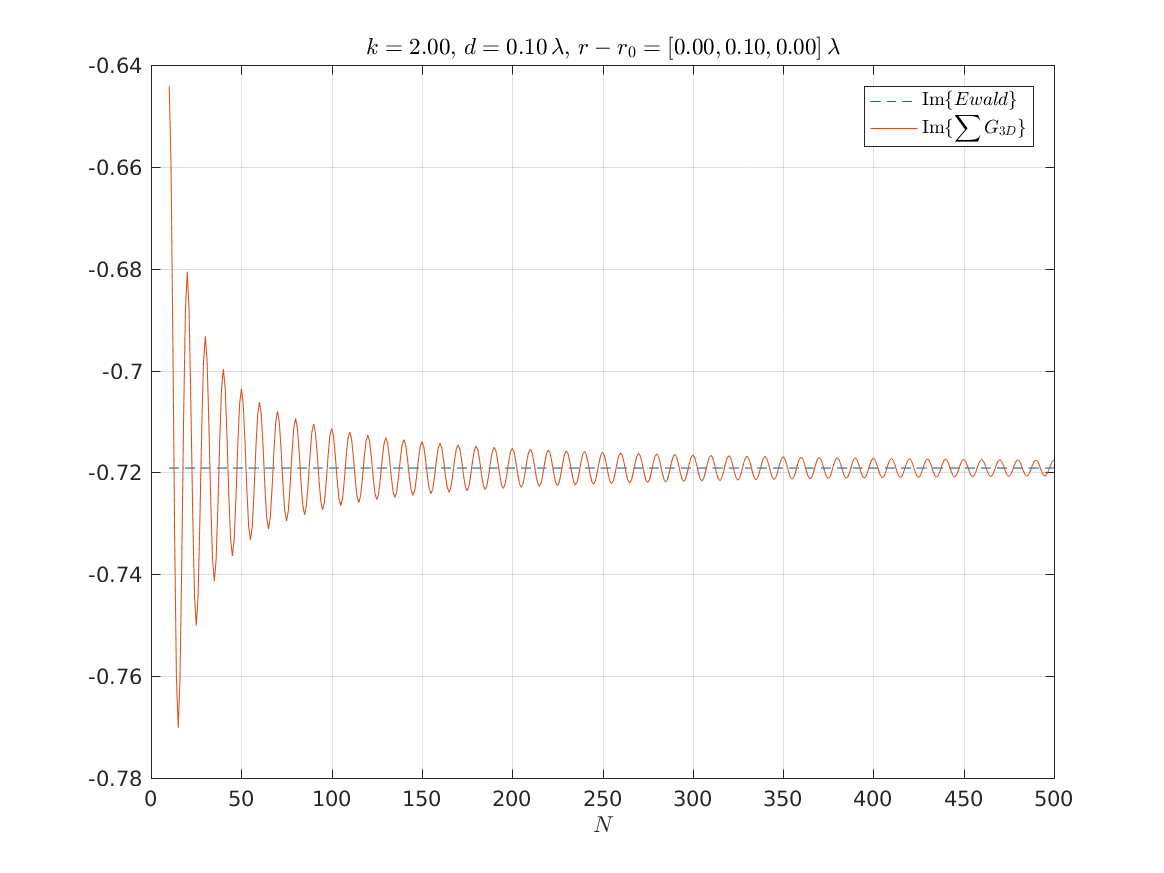
\includegraphics[width=0.8\textwidth]{GreenFunctions_convN_im_ew01.png}
\end{frame}
\begin{frame}{Dependence with frequency}
  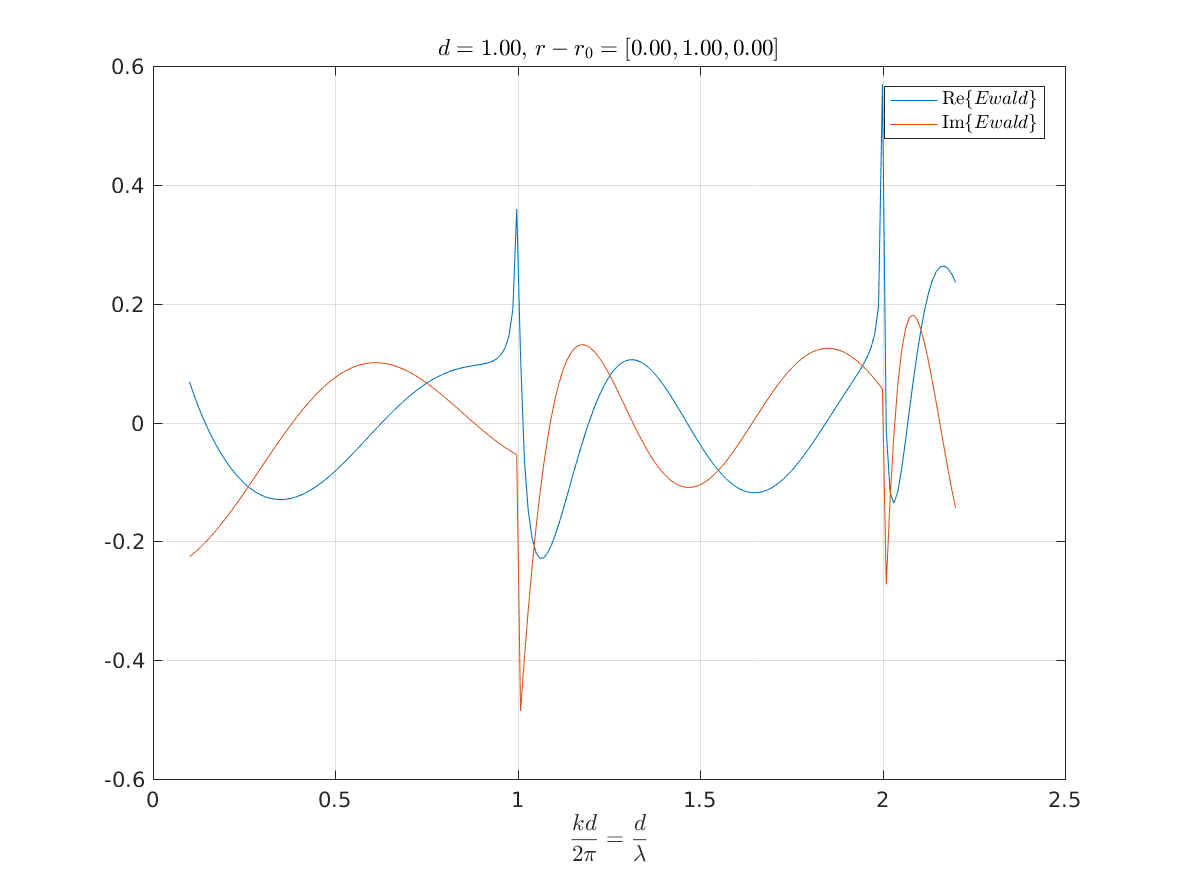
\includegraphics[width=0.9\textwidth]{GreenFunctions_ewald_k.png}
\end{frame}
\begin{frame}{Singularities when $\alpha_n^2 \to 0$}
  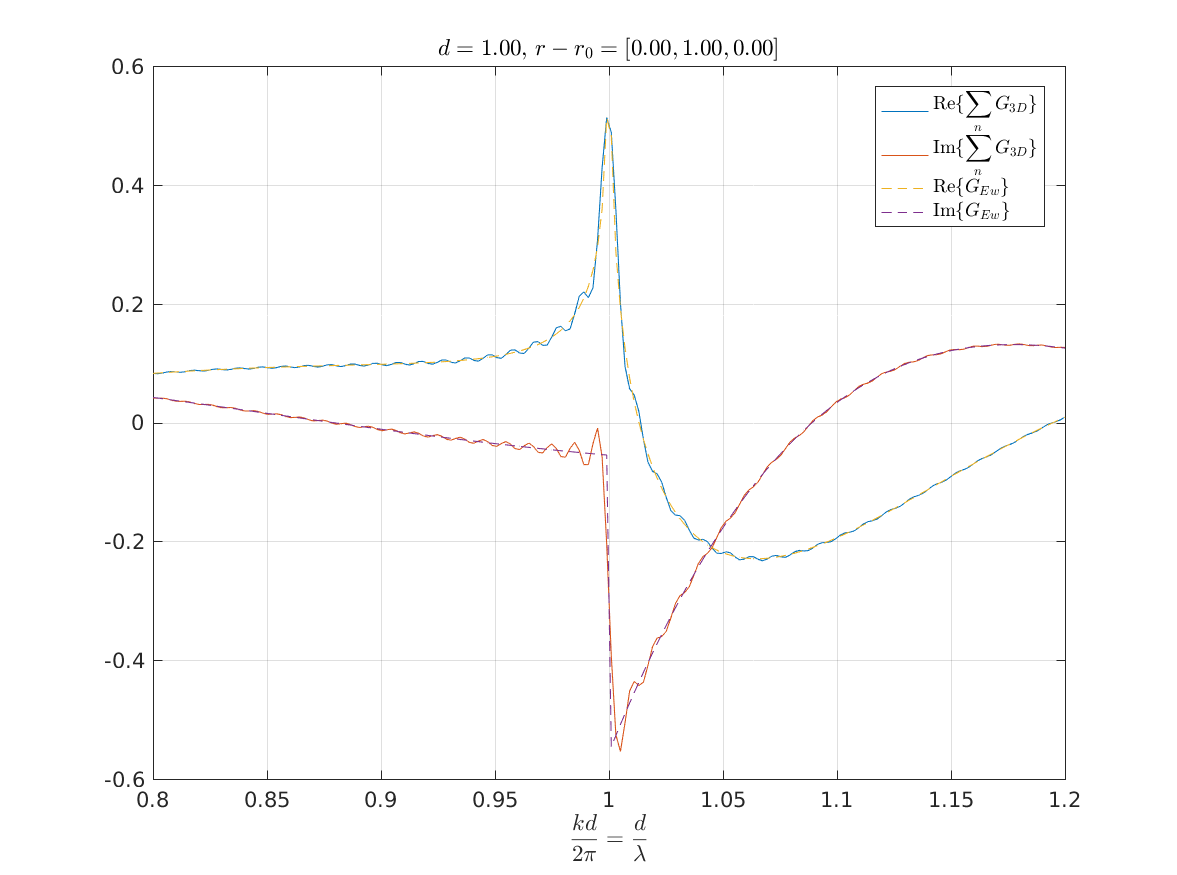
\includegraphics[width=0.9\textwidth]{GreenFunctions_ewald_k2.png}
\end{frame}

\begin{frame}{Additional notes}
  \begin{itemize}
    \item CPU time cost similar to sum 100 terms of $G_{3D}$.
    \item Matlab prototype.
    \item Numerical integral may be improved using classic algorithms for 
      calculate exponential integrals (see %
        \footnote{
          F. Capolino \emph{et al.}, ``Efficient Computation of the 2-D Green's 
          Function for 1-D Periodic Structures Using the Ewald Method'', 
          \emph{IEEE-TAP}, 2005. Equation (23).
        } and
        \footnote{
          F. Capolino \emph{et al.}, ``Efficient Computation of the 3D Green's 
          Function with One Dimensional Periodicity Using the Ewald Method'', 
          \emph{IEEE-APS}, 2006.
        })
      {\color{red} Done!: Calculation 10 times faster, but inestable for large 
      values of $\rho$ ($\rho>d$)}
    \item
      Checked:

      \[
        \int_{-\frac{d}{2}}^{\frac{d}{2}}
        G_{3D}(\rho,z)\, dz
        =
        G_{2D}(\rho)
      \]

      where $G_{3D}$ is numerically evaluated with Ewald, and $G_{2D}$ is the 
      Hankel function: 
      $\frac{1}{4j} H_0^{(2)}(k|\rho|)$.

  \end{itemize}
\end{frame}

% %%%%%%%%%%%%%%%%%%%%%%%%%%%%%%%%%%%%%%%%%%%%%%%%%%%%%%%%%%%%%%%

% %%%%%%%%%%%%%%%%%%%%%%%%%%%%%%%%%%%%%%%%%%%%%%%%%%%%%%%%%%%%%%%
  \subsection{Fortran Module}
% %%%%%%%%%%%%%%%%%%%%%%%%%%%%%%%%%%%%%%%%%%%%%%%%%%%%%%%%%%%%%%%

\begin{frame}[fragile,allowframebreaks]{Fortran Module}{\url{Ewald1D_Green_module.F90}}


  \begin{lstlisting}[style=myFORTRANcodeS]
MODULE Ewald1D_Green_module

   !> This module contains functions for evaluation different versions
   !> of the Green function.

   USE program_global_variables, ONLY : DBL, PI, ZERO, ONE
   USE program_global_variables, ONLY : HOFEM_LENGTH =>LENGTH
   USE program_global_variables, ONLY : MYEPS, MYEPS1, MYEPS2, MYEPS3, MYEPS6
   USE iso_fortran_env, ONLY : UNIT_OUT => OUTPUT_UNIT
   USE iso_fortran_env, ONLY : UNIT_ERROR => error_unit
   USE quadpack_double, ONLY : dqag, dqags, dqng, dlobatto 
   USE specfun_module, ONLY : vdExpIntP, dExpIntP, faddeeva_erfc
   USE specfun_module, ONLY : StruveH0 => STRVH0, StruveH1 => STRVH1

   !> IMPORTANT: Numerical stability concerns.
   PRIVATE
   PUBLIC :: g_integral_Ep, g_integral_IN, g_integral
   PUBLIC :: G1k_ewald, G2k_ewald
   PUBLIC :: Ewald1D_Green_function 

  \end{lstlisting}



\end{frame}


% %%%%%%%%%%%%%%%%%%%%%%%%%%%%%%%%%%%%%%%%%%%%%%%%%%%%%%%%%%%%%%%

\begin{frame}[fragile,allowframebreaks]{\url{Ewald1D_Green_function}}
  
  \begin{lstlisting}[style=myFORTRANcodeS]
      SUBROUTINE Ewald1D_Green_function &
            (K, Kz, rrp, slice_thickness, cylinder_axis, &
            G, dG, ddG)

         ! PARAMETERS
         REAL(KIND=DBL), PARAMETER :: RTOL = MYEPS2
         REAL(KIND=DBL), PARAMETER :: TOL = MYEPS

         ! INPUT:
         ! K: wavenumber
         ! Kz: transversal wavenumber to cylinder axis.
         !     Kz=cos(theta). Kz=0 for normal incidence
         ! rrp: vector r-r' in global coordinates
         REAL(KIND=DBL), INTENT(IN) :: rrp(3), K, Kz
         REAL(KIND=DBL), INTENT(IN) :: slice_thickness
         REAL(KIND=DBL), DIMENSION(3), INTENT(IN) :: cylinder_axis

         ! OUTPUT: complex green function value and derivatives
         COMPLEX(KIND=DBL), INTENT(OUT) :: G 
         COMPLEX(KIND=DBL), INTENT(OUT) :: dG(3)
         COMPLEX(KIND=DBL), INTENT(OUT) :: ddG(3,3)
  \end{lstlisting}

  Calculate:
  \[
    G_{p1D}(x_1,x_2,x_3)=\sum_n G(R_n) = \sum_n \hat{G}_1(k_n) + \sum_n G_2(R_n)
  \]
  where \((x_1,x_2,x_3)=\vec{r} - \vec{r'}\), and their derivatives:
  \[
    \frac{\partial G_{p1D}}{\partial x_i} \qquad \frac{\partial^2 G_{p1D}}{\partial x_i\partial x_j}
  \]

  \begin{itemize}\small
    \item Arbitrary periodicity axis ({\lstinline!cylinder_axis!}) 
    \item Sum convergence criteria defined by parameters:
      \begin{itemize}\footnotesize
        \item Relative: {\url{RTOL = MYEPS2}}
        \item Absolute: {\url{TOL = MYEPS2}}, {\url{tolabs = TOL*abs(G)}}
      \end{itemize}
      where {\lstinline!G!} is the value of the 2D Green function (Hankel function)
    \item Ewald separation constant: 
      {\url{E = sqrt(PI)/slice_thickness}}
      \begin{itemize}\footnotesize
        \item It is the recommended value by different authors (may not be the optimum)
      \end{itemize}
  \end{itemize}


\end{frame}

% %%%%%%%%%%%%%%%%%%%%%%%%%%%%%%%%%%%%%%%%%%%%%%%%%%%%%%%%%%%%%%%

\begin{frame}[fragile,allowframebreaks]{\url{G2k_ewald}}{Spatial sum element}
  
  \begin{lstlisting}[style=myFORTRANcodeS]
      SUBROUTINE G2k_ewald(rrp, K, E, &
            G2, dG2xyz, ddG2xyz)

         ! INPUT
         ! rrp: vector r - (r' + n*slice_thickness*cylinder_axis) 
         ! E: Separation constant in Ewald sum
         real(DBL), intent(in) :: rrp(3), K, E

         ! OUTPUT
         real(DBL), intent(out) :: G2, dG2xyz(3), ddG2xyz(3,3)
            
  \end{lstlisting}

  \vbs


  Calculate a term of the spatial sum: $G_2(R_n)$

  \begin{itemize}\small
    \item Complex erfc function calculated from Faddeeva function
      \begin{itemize}\footnotesize
        \item Algorithm ACM TOMS 680 (module \url{specfun_module.F90}) 
        \item Same algorithm that is used in Ewald 2D 
        \item \url{faddeeva_erfc} defined in \url{specfun_module.F90} 
      \end{itemize}
  \end{itemize}


\end{frame}

% %%%%%%%%%%%%%%%%%%%%%%%%%%%%%%%%%%%%%%%%%%%%%%%%%%%%%%%%%%%%%%%

\begin{frame}[fragile,allowframebreaks]{\url{G1k_ewald}}
  
  \begin{lstlisting}[style=myFORTRANcodeS]
      SUBROUTINE G1k_ewald(rho2, Az, vrho, K, Kz, floquet, &
            E, cylinder_axis, tolrel, tolabs, &
            G1, dG1xyz, ddG1xyz)

         ! INPUT
         ! Az: dot_product(r - r', cylinder_axis)
         ! vrho: r - r' - Az*cylinder_axis
         ! rho2: dot_product(vrho, vrho) 
         ! floquet: floquet wavenumber (2*Pi/slice_thickness*n)
         ! E: Separation constant in Ewald sum
         real(DBL), intent(in) :: rho2, Az, vrho(3)
         real(DBL), intent(in) :: K, Kz, floquet
         real(DBL), intent(in) :: E, cyl_axis(3)
         real(DBL), intent(in) :: tolrel, tolabs
         ! OUTPUT
         complex(DBL), intent(out) :: G1, dG1xyz(3), ddG1xyz(3,3)

         [...]
         flokz = floquet + kz
         alpha2 = (flokz**2 - k**2)/4.0_dbl
         a = alpha2/E**2
         b = rho2*E**2
         call g_integral(a, b,  1,   P, tolrel, tolabs,   err)
         call g_integral(a, b, -1,  dP, tolrel, tolabs,  derr)
         call g_integral(a, b, -3, ddP, tolrel, tolabs, dderr)
  \end{lstlisting}

  Calculate a term of the spatial sum: $\hat{G}_1(k_n)$

  \begin{itemize}\small
    \item It needs the following complex integral: 
      \[
        g(a,b,m) = \int_0^1 \frac{
          e^{-\frac{a}{z^2}-b z^2}
        }{z^m}
        \, dz
      \]
      where
      \begin{itemize}
        \item $a\in \mathbb{R}$, $b\in \mathbb{R^+}$
        \item $m \in \{1,-1,-3\}$
      \end{itemize}
  \end{itemize}

  \begin{columns}
    \column{0.45\linewidth}
    \begin{block}{\centering$a>0$}
      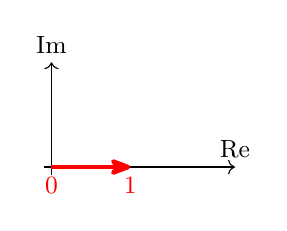
\begin{tikzpicture}[node font=\small]
        \draw[->] (-0.1,0) -- (2.33,0) node[above] {Re};
        \draw[->] (0,-0.1) -- (0,1.33) node[above] {Im};
        \draw[red, ultra thick, arrows={-Stealth[round]}] 
          (0,0) node [below] {$0$} 
        -- (1,0) node[below] {$1$}
        ;
      \end{tikzpicture}
    \end{block}
    \column{0.45\linewidth}
    \begin{block}{\centering$a<0$}
      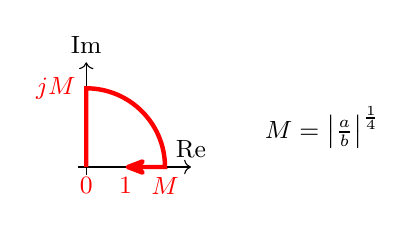
\begin{tikzpicture}[node font=\small]
        \draw[->] (-0.1,0) -- (1.33,0) node[above] {Re};
        \draw[->] (0,-0.1) -- (0,1.33) node[above] {Im};
        \draw[red, ultra thick, arrows={-Stealth[round]}] 
          (0,0) node [below] {$0$} -- (0,1) node[left] {$jM$} 
        arc[start angle=90, end angle=0, radius=1] node[below] {$M$}
        -- (0.5,0) node[below] {$1$}
        ;
        \node at (3,0.5) {$M=\left|\frac{a}{b}\right|^{\frac{1}{4}}$};
      \end{tikzpicture}
    \end{block}
  \end{columns}

  \vbss

  NOTE: If $m$ is even, the integral can be evaluated with the erfc function 
  (Ewald2D case)


\end{frame}

% %%%%%%%%%%%%%%%%%%%%%%%%%%%%%%%%%%%%%%%%%%%%%%%%%%%%%%%%%%%%%%%

\begin{frame}[fragile,allowframebreaks]{\url{g_integral}}
  
  \begin{lstlisting}[style=myFORTRANcodeS]
      SUBROUTINE g_integral(a, b, m, g, tolrel, tolabs, outerr, used_routine) 

         REAL(kind=DBL), PARAMETER :: EPS=MYEPS

         ! INPUT
         REAL(kind=DBL), INTENT(in) :: a, b
         INTEGER, INTENT(in) :: m
         REAL(kind=DBL), INTENT(IN) :: tolrel, tolabs
         ! OUTPUT
         COMPLEX(kind=DBL), INTENT(OUT) :: g
         REAL(kind=DBL), INTENT(OUT), OPTIONAL :: outerr
         INTEGER, INTENT(OUT), OPTIONAL :: used_routine
  \end{lstlisting}


  \begin{block}{Matlab implementation}
  \begin{lstlisting}[style=myFORTRANcodeS, language=Matlab]
  fun = @(x) exp(-( a./x.^2 + b*x.^2 ))./x.^m;
  if a>0
    g = integral(fun, 0, 1)
  else
    g = integral(fun, 0, 1, 'Waypoints', [Mmax*j, Mmax])
  end
  \end{lstlisting}
  \end{block}

\end{frame}

% %%%%%%%%%%%%%%%%%%%%%%%%%%%%%%%%%%%%%%%%%%%%%%%%%%%%%%%%%%%%%%%

\begin{frame}[fragile,allowframebreaks]{\url{g_integral_Ep}}{Alternative to numeric integration}

  \begin{lstlisting}[style=myFORTRANcodeS]
      SUBROUTINE g_integral_Ep(a, b, m, g, err, tolrel, abserr)
         ! Parameters
         INTEGER, PARAMETER :: MAXITER = 10000
  \end{lstlisting}
  
  \vbs

  \begin{itemize}\small
    \item Based on \href{https://dlmf.nist.gov/6.2}{\emph{exponential integral}}
    \item Faster than numerical integration
    \item Calculated by MKL function \url{vdExpInt1} 
    \item Details:
      \begin{columns}
        \column{0.8\linewidth}
        \begin{block}{}\footnotesize
          F. Capolino \emph{et al.}, ``Efficient Computation of the 2-D Green's 
          Function for 1-D Periodic Structures Using the Ewald Method'', 
          \emph{IEEE-TAP}, 2005.
        \end{block}{}
      \end{columns}
      \vbss
    \item Numerical problems when $b \gg 1$ or $a \ll -1$ or $|ab| \gg 1$ or ...

  \end{itemize}

\end{frame}

% %%%%%%%%%%%%%%%%%%%%%%%%%%%%%%%%%%%%%%%%%%%%%%%%%%%%%%%%%%%%%%%

\begin{frame}[fragile,allowframebreaks]{\url{g_integral_IN}}{Numeric integration}

  \begin{lstlisting}[style=myFORTRANcodeS]
      SUBROUTINE g_integral_IN(a, b, m, gI, err, tolrel, tolabsd)
         ! Parameters
         REAL(KIND=DBL), PARAMETER :: EPS = MYEPS1
         REAL(KIND=DBL), PARAMETER :: LOGEPS = log(1/EPS)
         ! INPUT
         real(kind=DBL), intent(in) :: a, b
         integer, intent(in) :: m
         real(kind=DBL), intent(in) :: tolrel
         real(kind=DBL), OPTIONAL :: tolabsd
         ! OUTPUT
         COMPLEX(kind=DBL), INTENT(OUT) :: gI
         REAL(kind=DBL), INTENT(OUT) :: err
  \end{lstlisting}
  

  \begin{itemize}\small
    \item Complex integration on liner paths:
      \begin{itemize}\small
        \item The result is real. It is a real integration.
        \item The integrand is smooth.
        \item The simple real integration function \url{dqng} from library 
          \href{https://github.com/jacobwilliams/quadpack}{\emph{quadpack2}} is used.
      \end{itemize}
    \item Integration on circular path:
      \begin{itemize}\small
        \item Integrand oscilate (more when $b \gg 1$)
        \item Imaginary part: is a Bessel function
        \item Real part: is a \href{https://dlmf.nist.gov/11.2}{Struve function}.
      \end{itemize}
  \end{itemize}
  

\end{frame}

% %%%%%%%%%%%%%%%%%%%%%%%%%%%%%%%%%%%%%%%%%%%%%%%%%%%%%%%%%%%%%%%

\begin{frame}[fragile,allowframebreaks]{\url{g_integral_IN}}{Integration on circular part}
  \begin{lstlisting}[style=myFORTRANcodeS]
            ! Integral from j*Mmin  to Mmin (circular path)
            if (m==1) then
               gIaux = -PI/2.0_dbl*StruveH0(ab)
            elseif (m==-1) then
               gIaux = Mmin2*(1.0_dbl - PI/2.0_dbl*StruveH1(ab))
            elseif (m==-3) then
               gIaux = Mmin4*PI/2.0_dbl*(StruveH0(ab) - 2.0_dbl*StruveH1(ab)/ab)
            else
               call dqng(g_integrand_circle_real, PI/2.0_dbl, 0.0_dbl, tolabs, tolrel, gIaux, erraux, neval, ier)
               err = err + erraux
            end if
            gI_real = gI_real + gIaux
            [...]
            
            ! Imaginary part
            gI_imag = - PI/2*(-a)**(p-1)* & 
               BESSEL_JN(p-1, 2*sqrt(abs(a*b))) &
               /sqrt(abs(a*b))**(p-1)
  \end{lstlisting}
\end{frame}

% %%%%%%%%%%%%%%%%%%%%%%%%%%%%%%%%%%%%%%%%%%%%%%%%%%%%%%%%%%%%%%%

\begin{frame}[fragile,allowframebreaks]{\url{specfun_module}}{Integration on circular part}
  \begin{lstlisting}[style=myFORTRANcodeS]
MODULE specfun_module

   !> This module contains tools for evaluate special functions

#define CHKERRQ(n,x) IF (n /= 0) THEN; WRITE(UNIT_OUT,*) 'ERROR: ',x;STOP; ENDIF

   USE program_global_variables, ONLY : DBL, PI, ZERO, ONE
   USE program_global_variables, ONLY : MYEPS, MYEPS1, MYEPS2, MYEPS3, MYEPS6
   USE iso_fortran_env, ONLY : UNIT_OUT => OUTPUT_UNIT

   IMPLICIT NONE

   PRIVATE
   PUBLIC :: vdExpIntP, dExpIntP
   PUBLIC :: faddeeva_erfc
   PUBLIC :: STRVH0, STRVH1 
   PUBLIC :: STVH0, STVH1 

   include "mkl_vml"
  \end{lstlisting}
  
  \begin{lstlisting}[style=myFORTRANcodeS]

      !------------------------------------------------------------------
      !> @author
      !> Sergio Llorente Romano, Luis E. Garcia Castillo, Adrian Amor
      !
      !  DESCRIPTION:
      !> Struve function H0 and H1
      !> 
      !> Adaption from https://netlib.org/toms/757 
      !>
      !------------------------------------------------------------------
      
      FUNCTION STRVH0(XVALUE)
      [...]
      FUNCTION STRVH1(XVALUE)
   
  \end{lstlisting}
\end{frame}
